\documentclass[11pt,traditabstract]{article}
\usepackage{geometry}                
\geometry{letterpaper} 
\usepackage{graphicx}
\usepackage{amssymb}
\usepackage{epstopdf}
\usepackage{amsmath}
\usepackage{morefloats}
\usepackage{hyperref}
\usepackage[round]{natbib}
\geometry{margin=1in}
\DeclareGraphicsRule{.tif}{png}{.png}{`convert #1 `dirname #1`/`basename #1 .tif`.png}
\graphicspath{{../../scuffCode/CubeSphere/}{../../scuffCode/CubeSphereAspect/}{../../scuffCode/CubeSphereDepth/}{../../scuffCode/Comparison/}{../../scuffCode/CubeSphereBest/}{../../scuffCode/CubeSphereLateral/}{../../scuffCode/Geometry/}}

\newcommand{\E}{\mathcal{E}}
 
\title{\vspace{-0.5in}Internal Note: The Casimir Force in a \\ Micron-Scale Optical Trap Geometry}
\author{Noah Kurinsky}
%\date{}                                  

\begin{document}
\maketitle

\begin{abstract}
This document explains the recent theory and numerical methods relevant to computing the casimir force in our geometry. I will cover the historical analytical solutions, and then focus on the new scattering theory, discussing various techniques needed in different regimes. I then present the best numerical result from our geometry and discuss uncertainty. The overall purpose of this document is to summarize our knowledge of Casimir forces within the sphere-cantilever geometry, and compile useful literature for robust comparison of our eventual measurements to existing theory. I also try to make explicit the connection between the microscopic and macroscopic descriptions of the Casimir force, corresponding generally to the comparison of the particulate and field descriptions, quantum mechanically.
\end{abstract}

\section{Background}

The Casimir effect rises from zero-point energy fluctuations between conducting surfaces, which can be thought of as a result of positive feedback between stochastic deviations from the nominally non-polarized state. A good description of this is provided by \citet{rodr}, reproduced here:
\begin{quote}
Van der Waals forces are a familiar concept from introductory physics and chemistry: two neutral particles have fluctuating dipole moments resulting from quantum or thermal effects, which, for a particle separation of d, lead to a $d^{-6}$ interaction energy that is commonly used, for example, as a long-range attraction term when describing the interactions between atoms and molecules. Whenever one particle acquires a spontaneous dipole moment $\mathbf{p1}$, the resulting dipole electric field polarizes the adjacent particle to produce an induced dipole moment $\mathbf{p2}\sim d^{-3}$. Assuming positive polarizabilities, the direction of the dipole fields means that these two dipoles are oriented so as to attract each other, with an interaction energy that scales as $d^{-6}$. This leads to the van der Waals `dispersion' force, and similar considerations apply to particles with permanent dipole moments that can rotate freely. The key to more general considerations of Casimir physics is to understand that this $d^{-6}$ picture of van der Waals forces makes two crucial approximations that are not always valid: it employs the quasi-static approximation to ignore wave effects, and also ignores multiple scattering if there are more than two particles.

The quasi-static approximation assumes that the dipole moment $\mathbf{p1}$ polarizes the second particle instantaneously, which is valid if $d$ is much smaller than the typical wavelength of the fluctuating fields. However, the finite wave propagation speed of light must be taken into account when d is much larger than the typical wavelength, and it turns out that the resulting Casimir-Polder interaction energy asymptotically scales as $d^{-7}$ for large $d$. More generally, the interaction is not a simple power law between these limits, but instead depends on an integral of fluctuations at all frequencies scaled by a frequency-dependent polarizability of the particles.

The presence of multiple particles further complicates the situation because multiple scattering must be considered. For example, with three particles, the initial dipole $\mathbf{p1}$ will induce polarizations $\mathbf{p2}$ and $\mathbf{p3}$ in the other two particles, but $\mathbf{p2}$ will create its own field that further modifies $\mathbf{p3}$, and so on. Thus, the interaction between multiple particles is generally non-additive, and there is no two-body force law that can simply be summed to incorporate all interactions. Multiple scattering is negligible for a sufficiently dilute gas or for weak polarizabilities, but it becomes very significant for interactions between two (or more) solid bodies, which consist of many fluctuating dipole moments that all interact in a complicated way through electromagnetic radiation. When these multiple scattering effects are combined with wave retardation in a complete picture, they yield the Casimir force.

Hendrik Casimir based his prediction on a simplified model involving two parallel perfectly conducting plates separated by a vacuum. Although the Casimir force arises from electromagnetic fluctuations, real photons are not involved. Quantum mechanically, these fluctuations can be described in terms of virtual photons of energy equal to the zero-point energies of the electromagnetic modes of the system. By considering the contribution of the electromagnetic field modes to the zero-point energy of the parallel plate configuration, Casimir predicted an attractive force between the plates. Because only electromagnetic modes that have nodes on both walls can exist within the cavity, the mode frequencies ($\omega$) depend on the separation between the plates, giving rise to a pressure $P_C$. The force in this case is attractive because the mode density in free space is larger than that between the plates. Following Casimir's calculation, Lifshitz, Dzyaloshinski and Pitaveski considered the more general case of realistic dielectric plates by exploiting the fluctuation-dissipation theorem, which relates the dissipative properties of the plates (that is, the optical absorption resulting from the many microscopic dipoles in the plates) and the resulting electromagnetic fluctuations at equilibrium. For realistic metallic plates separated by d, the force again scales as $d^{-4}$ for large $d.$ At small $d$, the force scales as $d^{-3}$ (this is the quasi-static limit, where the coefficient is known as the Hamaker constant), with a complicated intermediate $d$-dependence that is determined by the frequency-dependent permittivity ($\epsilon$) of the materials. Here, `small' and `large' $d$ are relative to a characteristic wavelength $\lambda_0$, which for metals is the plasma wavelength and is typically in the ultraviolet range (a few hundred nanometres). The geometry of the system can be used to greatly modify wave propagation beyond the simple planar regime, but a broad-bandwidth scattering calculation is required to capture the complete physics of such interactions.
\end{quote}

The nominal quantity computed in analysis of this effect is the casimir energy as a function of separation between metallic reflectors. In Casimir's classical result \citep{Casimir} the energy between two parallel perfectly conducting plates was calculated exactly to be \citep[given in nice form by][]{ScatteringTheory}
$$
\E=-\frac{\hbar c\pi^2A}{720L^3}
$$
which of course makes the Casimir pressure between the two plates
$$
P_C=\frac{1}{A}\frac{d\E}{dL}=\frac{\hbar c\pi^2}{240L^4}
$$
and thus in vacuum, two perfectly conducting plates at $T=0K$ will attract each other with a pressure independent of plate area. This geometry has since been studied in various limits, including most notably finite conductivity and temperature \citep[][ and references therein]{ScatteringTheory} but also finite extent and non-planar geometries \citep[][ and references therein]{Rahi}.

Despite the theoretical interest, the difficulty inherent in measuring the Casimir force prevented precise measurement until the landmark work of \citet{Lamoreaux}, who measured the force between a plate and a curved surface, to confirm the theory based on small approximations to the classical model. In this geometry, the Casimir force became an attraction with a magnitude of tens of micro dynes at separations of a few micrometers, for a plate and a small curved surface with radius of curvature of about 10cm. This work helped to solidify the theory behind finite-conductivity corrections, thermal corrections, and verify a long-used approximation called the Proximity Force Approximation (PFA, see next section) which has been used to calculate the Casimir force in nearly parallel geometries. More recent work performed this verification with parallel planes, a much more difficult measurement due to the requirement of static parallel configuration between planes, the motivation for the curved-planar geometry \citep{rodr}.

In geometries which deviate from the non-ideal case, the calculation of the Casimir force becomes highly non-trivial. The PFA, for example, assumes that in the nearly planar limit, the Casimir force can be computed as the superposition of forces from all sets of nearly parallel subsections of the curved surface directly opposite the planar surface. It is widely known that this approximation only holds in the the limit of large curvature compared to distance, and thus for a sphere with curvature radius equal to or less than the separation between surfaces, the only analytical expression for this force is no longer strictly valid.

In the context of this experiment, this is the main barrier preventing us from producing a quick prediction for the Casimir force. Our geometry is neither spherically nor cylindrically symmetric, as the cantilever we use as a force probe has a rectangular cross-section with one dimension much longer than the other, and the sphere is much smaller than typical separations. In addition, our cantilever is silicon coated in gold, and our bead is made of silica, whereas the normal materials dealt with are conductors thick enough that only one material correction needs to be made. Finally, we operate the bead at non-zero temperature, which requires temperature corrections which are non-trivial in the non-parallel geometry. Despite the barrier to computation of the force, it should in principle be easy to measure if we can understand the systematic effects inherent to our geometry; this is the motivation behind this note. In addition, it will most likely represent the main background we must compensate for in the measurement of other sub micron forces, namely non-newtonian gravitational corrections and chameleon models of dark energy.

In this note, I will outline the steps taken in attempting to predict the magnitude of the Casimir force we expect to measure in our experiment, beginning with the PFA, expansions to the PFA, and other simple analytical solutions. I will then cover the finite conductivity and temperature corrections, and then discuss the exact analytic and numerical solutions which exist to compensate for these non-idealities. I will present predictions, and discuss other approaches we have attempted and potential limitations of the calculations. The idea will be that it is left up to those more theoretically inclined to compute the exact theoretical prediction to our model, but that we should be able to come up with a prediction to within 10-20\% of the true Casimir force as a function of distance. I will conclude by discussing the reason for the limitations and assumptions.

\pagebreak
\section{Analytical Solutions}

The only exact solutions come for the parallel plane solution as initially derived by Casimir \citep{Casimir} for a perfect electrical conductor (PEC), and later for finite conductivity, multilayer films, and extended geometries \citep{rodr}. Casimir's original formula was presented in the previous section. To extend this analytical solution to arbitrary situations, one has to correct for a wide range of effects, including
\begin{itemize}
\item Non-Planar Geometry
\item Compact Geometry
\item Finite Conductivity
\item Finite Temperature
\item Asymmetry
\end{itemize}
Of these effects, the first, third, and fourth were historically first to be attempted, but until recently asymmetric geometries and compact geometries were not generally explored. The recent theoretical progress in this area has been focused on determining a general framework by which, in any arbitrary configuration, the calculation resulting in the Casimir force can be constructed from the framework of scattering theory, largely within electromagnetism rather than quantum field theory. Good references for this scattering theory approach include \citet{ScatteringTheory}, \citet{Emig07}, and \citet{Rahi}. These papers come from two distinct theory groups, one in France (Lambrecht et. al.) and one at MIT (Kardar, Jaffe, Emig et. al) who have separately developed this theory and contributed synergistically to the effort. The group in France come from a more experimental angle, which the MIT group comes from a more pure theory standpoint.

\subsection{Proximity Force Approximation (PFA)}

\begin{figure}[!h]
\centering
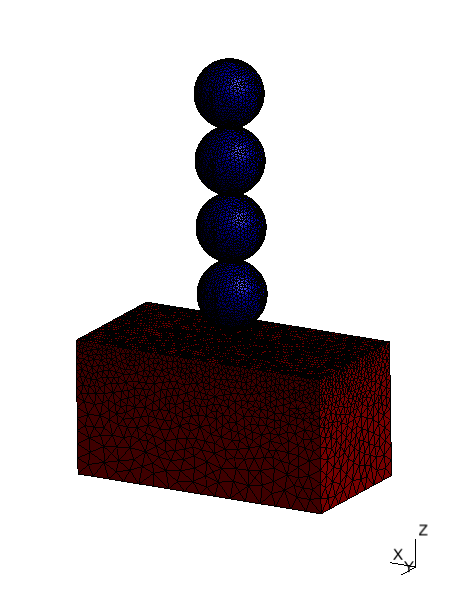
\includegraphics[height=3in]{geometry}
\caption{Geometry of cantilever and bead, truncated in the x direction and limited to tens of plasma wavelengths in depth. Here we show four distances of the bead from the cantilever in the z direction.}\label{fig:geo}
\end{figure}

Consider the geometry shown in figure \ref{fig:geo}. This is clearly not the case derived by Casimir, and even for the closest separation of sphere from plane, neither object can be though of as extended. Remembering, however, that Casimir forces scale as $d^{-4}$, given one surface much closer to another than the scale length of its physical distortion, one might postulate that, if the separation along the $z$ axis is small enough, we could approximate the Casimir force as the sum of forces from each pair of opposite faces, approximately stated to be parallel. In integral form, this is \citep{Dexp}
$$
E_{C}\approx E_{PFA}=\int_{\Sigma}E_{pp}(z)d\sigma
$$
where $E_{pp}$ is the Casimir energy per unit area of two parallel planes separated by a distance $z$, using the normal Casimir equation from the previous section. Here, the geometric argument that surfaces be approximately parallel, and forces additive, corresponds to the limit $R>>d$. For the sphere plane geometry, this integral yields the formula \citep{Durand}
$$
F_{PFA}=2\pi R \frac{E_C}{A}=\frac{\hbar c\pi^3R}{360L^3}
$$
or in terms of energy,
$$
E_{PFA}=-\frac{\hbar c\pi^3R}{720L^2}
$$
The PFA is based on the more general Derjaguin approximation for distance dependent forces between planar and curved surfaces, as discussed in \citet{BeyondPFA}. Because of the crucial assumption that the Casimir force obey the superposition principle, which it will not, in general, this is an uncontrolled approximation, as discussed in \citet{Emig07}, but the PFA has been shown to work well within its limit of applicability; figure \ref{fig:LamPFA} was calculated using the PFA, and matches the data measured by \citet{Lamoreaux} nearly perfectly.

\subsection{Expanded Proximity Force Approximation}

To obtain a better picture of the Casimir force, and a more robust theory, we need to discuss a more general framework for calculating Casimir forces. The scattering theory framework for Casimir calculations is discussed at length in \citet{ScatteringTheory}, \citet{Emig07}, and \citet{Rahi}. The general idea is to treat the space between two surfaces as a cavity in which imaginary photons propagate, and calculate the force due to allowable modes of virtual photons across all separations within the cavity. From \citet{Rahi} and \citet{Emig07}, we find that the expression for Casimir energy between any number of arbitrary surfaces is given by
$$
E=\frac{\hbar c}{2\pi}\int_0^{\infty}d\kappa\ln\frac{\det{\mathbb{M}}}{\det{\mathbb{M}_{\infty}}}
$$
where $\mathbb{M}$ is a modified scattering matrix derived in \citet{Emig07} and $\kappa$ is imaginary frequency, the continuous zero-temperature limit of the Matsubara sum, discussed in the next section. 

I write this somewhat obscure integral to provide a starting point for future more targeted numerical computations, pointing out that these scattering matrices are very large, and integrating their determinants corresponds to diagonalizing and integrating functions of $\kappa$. The numerical code I discuss later on is essentially a means by which arbitrary geometries can be translated into these scattering matrices, after which the code attempts to diagonalize these matrices and perform this integral. If we could exploit any particular symmetry in our geometry to expedite the calculation over the most brute-force approach, this would be an avenue by which more efficient numerical calculations could proceed.

Following this theory, many recent efforts have focused on using this formalism to work out corrections to the PFA \citep[see e.g.][]{Dexp, Bimonte12, Bulgac, Durand}. \citet{Emig07} extensively explored expansions in the small and large distance regimes for the sphere-plate geometry for a perfectly conducting plate, and found an analytical solution for far distances, and a power-law fit to PFA corrections for small distances, which I have stitched together to form a prediction curve over all separations (\citet{Emig07} used mathematica to numerically integrate this geometry over the whole range, verifying continuity between the two expressions). 

At small distances, the empirical power series fit of the correction to the PFA (accurate to $0.15R$ in face-to-face separation between plate and sphere) is
$$
\frac{E}{E_{PFA}}=1+\theta_1\frac{d}{R}+\theta_2\left(\frac{d}{R}\right)^2+\mathcal{O}\left[\left(\frac{d}{R}\right)^3\right]
$$
where the numerically fitted parameters are \citep{Emig07} are
$$
\theta_1=-1.42\pm0.02 \;\;\;\;\; \theta_2=2.39\pm0.14
$$
The semi-analytic expansion for the large distance limit ($d>2R$)
$$
E=\frac{\hbar c}{\pi}\frac{1}{L}\sum_{j=4}^\infty b_j\left(\frac{R}{L}\right)^{j-1}
$$
with the coefficients
$$
b_4=-\frac{9}{16} \;\;\; b_5=0 \;\;\; b_6=-\frac{25}{32} \;\;\; b_7=-\frac{3023}{4096}
$$
$$
b_8=-\frac{12551}{9600} \;\;\; b_9=\frac{1282293}{163840} \;\;\; b_{10}=-\frac{32027856257}{722534400} \;\;\; b_{11}=\frac{39492614653}{412876800}
$$
these expressions are plotted in figure \ref{fig:expansion}. The empirical fit at small separations was also explored comparably by \citet{BeyondPFA}. These expressions still assume perfect conductivity, zero temperature, and infinite plane surface, but these can be formulated as additional multiplicative corrections.

\begin{figure}[!h]
\centering
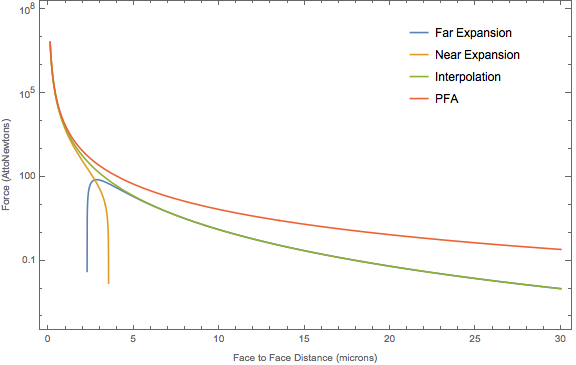
\includegraphics[height=4in]{analytical}
\caption{Full length scale calculation for casimir force in plane-sphere configuration, for infinite conductivity and zero temperature, compared to PFA.}\label{fig:expansion}
\end{figure}

\citet{Durand} explore geometry effects as a function of radius and separation, and tabulate corrections based on face to face separation, but their estimates are for infinite planes and do not extend far enough from the plane to be practically useful for our predictions. I have plotted corrections for the various numerically computed geometries in figures below as a function face to face separation in figures \ref{fig:geometric} and \ref{fig:geometricbest}. Arguments based on fractional area covered  

\subsection{Finite Conductivity Corrections}
This section follows from \citet{Lambrecht} \citep[see also][]{BeyondPFA}. Recognizing that the integral above is of scattering matrices over frequency space, the conductivity will factor into the scattering matrix for a given frequency and affect the overall Casimir energy. Another way to think about this is that, in our dipole metaphor, different elements have different polarizabilities and will react with different characteristic frequencies to perturbations.

The dielectric constant is large at frequencies smaller than the plasma frequency $\omega_p$, so corrections are more relevant at separations smaller than the plasma wavelength
$$
\lambda_p=\frac{2\pi c}{\omega_p}
$$
where
$$
\omega_p^2=\frac{Nq^2}{\epsilon_0m^*}=\frac{ZN_aq^2}{\epsilon_0m^*}=\frac{\rho q^2}{\epsilon_0m^*m_z}
$$
and in turn, $N$ is the number of conduction electrons per unit volume, $Z$ is the number of free electrons per atom (taken to just be $Z=1$), $N_a$ is the atomic number density, $q$ is the electron charge, and $m^*$ is effective electron mass, also taken to be 1 for Au though not necessarily for $\mathrm{SiO^2}$. We in turn calculate $N_a$ as the density $\rho$ divided by the atomic mass $m_Z$ for the species.

The correction due to conductivity is parameterized as
$$
F_{finite}=\eta_{E}F_{infinite}
$$
where the reduction factor for the Casimir energy is given by \citep{Lambrecht}
\begin{equation}
\eta_E=-\frac{180L^3}{c\pi^4}\int^{\infty}_{0}\kappa d\kappa\int^{c\kappa}_0\sum_{p=\parallel,\perp}\log{\left(1-r_{p,1}(i\omega,i\kappa)r_{p,2}(i\omega,i\kappa)e^{-2\kappa L}\right)}d\omega
\end{equation}
where $r_{p,i}(i\omega,i\kappa)$ is the reflection amplitude of surface $i$ for polarization $p$, where $i\omega$ is the imaginary frequency and $i\kappa$ is the imaginary wave vector along the longitudinal direction of the cavity, or the normal to the plane. The reflection coefficients for thick slabs are given by
\begin{align}
r_{\perp}&=-\frac{\sqrt{\omega^2(\epsilon(i\omega)-1)+c^2\kappa}-c\kappa}{\sqrt{\omega^2(\epsilon(i\omega)-1)+c^2\kappa}+c\kappa} \\
r_{\parallel}&=\frac{\sqrt{\omega^2(\epsilon(i\omega)-1)+c^2\kappa}-c\kappa\epsilon(i\omega)}{\sqrt{\omega^2(\epsilon(i\omega)-1)+c^2\kappa}+c\kappa\epsilon(i\omega)}
\end{align}
\citet{Lambrecht} suggest numerical integration over the range $10^{-4}$ to $10^{3}$ eV for distances 0.1 to 10 $\mu$m for best efficiency in numerics, though in mathematica the integral converges fairly quickly (see the mathematica notebook for the implemented function).

The non-trivial aspect of this correction is the form of $\epsilon(i\omega)$. From \citet{Lambrecht}, we see that there are two main options for how to evaluate this function, namely empirical measurements or through a model. The two dominant models are the plasma and Drude models of conductivity, which do not agree and are a major source of disagreement in current literature (this is one motivation for performing measurements of the thermal casimir force). The plasma model gives
$$
\epsilon(i\omega)=1+\frac{\omega_p^2}{\omega^2}
$$
while the Drude model adds the relaxation parameter $\gamma$, using the form
$$
\epsilon(i\omega)=1+\frac{\omega_p^2}{\omega(\omega+\gamma)}
$$
For gold, we find $\omega_p\approx1.37*10^{16}$ and $\gamma\approx4.521*10^{13}$. For the numerical calculations here, I employed Drude model, as \citet{Lambrecht} suggests it is a better fit to the empirical data, but the main correction comes from the silica bead, which follows the dielectric form
$$
\epsilon(i\omega)=\epsilon_{\infty} + \frac{\epsilon_{0} - \epsilon_{\infty}}{1 - \frac{\omega^2}{\omega_p^2}}
$$
where $\epsilon_0$ and $\epsilon_\infty$ are permittivities above and below the divergent pole at $\omega_p$. This is the form used in an example calculation which came with the numerical code, and could be refined further, though it does seem to be approximately correct. A good first reference, which has a similar form, would be \citet{Silica}. The values used for these calculations were $\epsilon_0\approx 11.87$, $\epsilon_\infty\approx1.035$, and $\omega_p\approx 8.86*10^{15}$. 

\subsection{Temperature Corrections}

The length at which the thermal casimir force becomes relevant is determined by the thermal length scale,
$$
\lambda_T=\frac{\hbar c}{k_B T}
$$
and the robust way to incorporate this into the calculation is to evaluate the integral as an infinite sum over the Matsubara frequencies
$$
\xi_n=\frac{2\pi n k T}{\hbar}
$$
as discussed in \citet{Durand}. Another robust improvement on these estimates would be to evaluate the integral numerically in this way.

\begin{figure}[h]
\centering
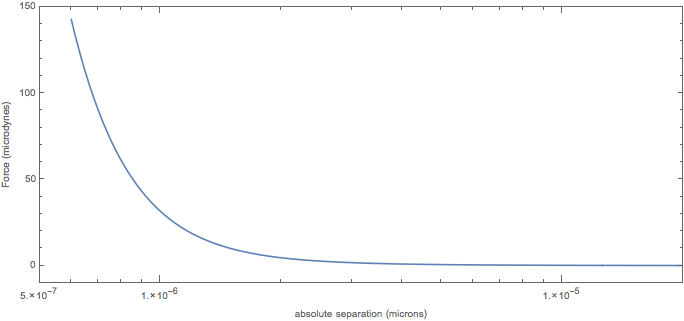
\includegraphics[width=5in]{LamPFA}
\caption{Reproduced calculation of PFA from \citet{Lamoreaux}}\label{fig:LamPFA}
\end{figure}

Following \citet{Lamoreaux}, we choose to instead multiply the zero temperature force by a semi-analytic correction factor 
$$
F_T=\eta_TF_0
$$
where
$$
\eta_T=1+\frac{720}{\pi^2}\left\{\begin{array}{l r}
1.202(\xi^3/2\pi)\zeta(3)-(\xi^4\pi^2/45)&\xi\le1/2 \\
1.202(\xi/8\pi)\zeta(3)-(\pi^2/720)&\xi < 1/2
\end{array}\right.
$$
where $\xi=kTL/\hbar c$ is the length scale from the Matsubara sum. This correction is trusted given that, using this temperature correction and the PFA, I was able to reproduce the force curve which matched the data points from this casimir force measurement. This plot can be seen in figure \ref{fig:LamPFA}.

\subsection{Expected accuracy}
While we are limited in the accuracy of our analytic calculations by assumptions of infinite plane and uncertain model of conductivity, we can expect these calculations to be nearly exact for small values of $d/R$, given that the PFA alone is exact there, and reasonably should expect to obtain results within an order of magnitude of the true force for the largest separations. Major sources of uncertainty include temperature corrections and dielectric corrections, as well as uncertainty in the parameters of the fitted power series approximation and in the interpolated range between this power series and the analytic solution. Much of this uncertainty comes from using multiplicative corrections to the integral solution found for special conditions, and as such more accurate predictions could be obtained from numerically performing this integral; this is what is done in the next section.

\section{Numerical Computation}

We employed the Scuff-EM cas3d program\footnote{\url{http://homerreid.dyndns.org/scuff-EM/scuff-cas3D/}}\citep{Cas3DPRL,Cas3DPRA}, which numerically evaluates the integral from the previous section for arbitrary geometries, conductivities, and temperatures. The main challenge was to create a geometry whose BEM matrix was diagonalizable in a reasonable amount of time without sacrificing accuracy. Early convergence tests with a very large and uniformly gridded cantilever showed that the length scale of the gridding was important in the convergence of the prediction (figure ref{fog:conv1}). The earlier predictions did not converge properly as a function of radius, performing poorly except around 1 micron, as seen in figure \ref{fig:earlyEstimate}. 

\begin{figure}[!h]
\centering
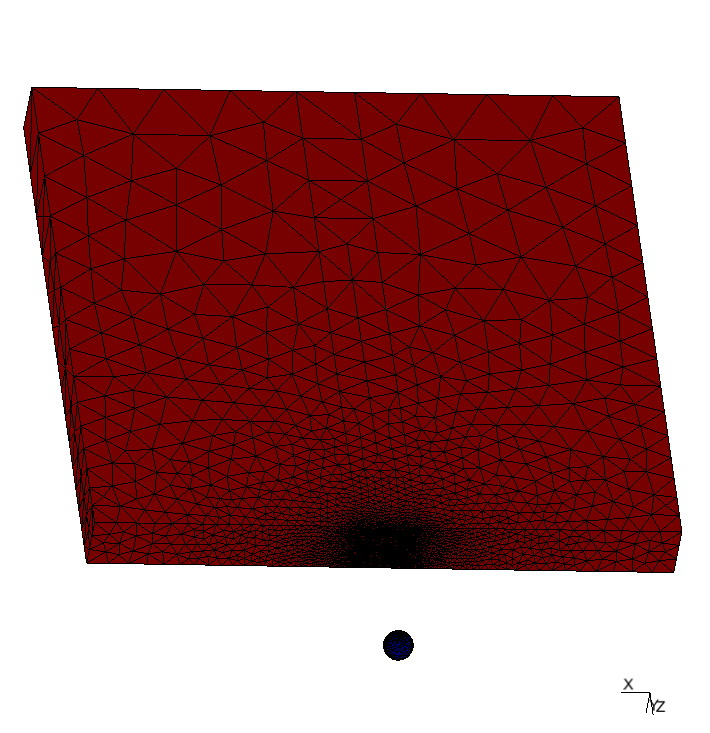
\includegraphics[height=3in]{Bead_positions}
\caption{Geometry of cantilever and bead, representing the full x-y shape of the cantilever and extended to ~100 plasma wavelengths in depth. Here we show the bead 20 microns from the cantilever in the z direction.}\label{fig:geoLarge}
\end{figure}

\begin{figure}[!h]
\centering
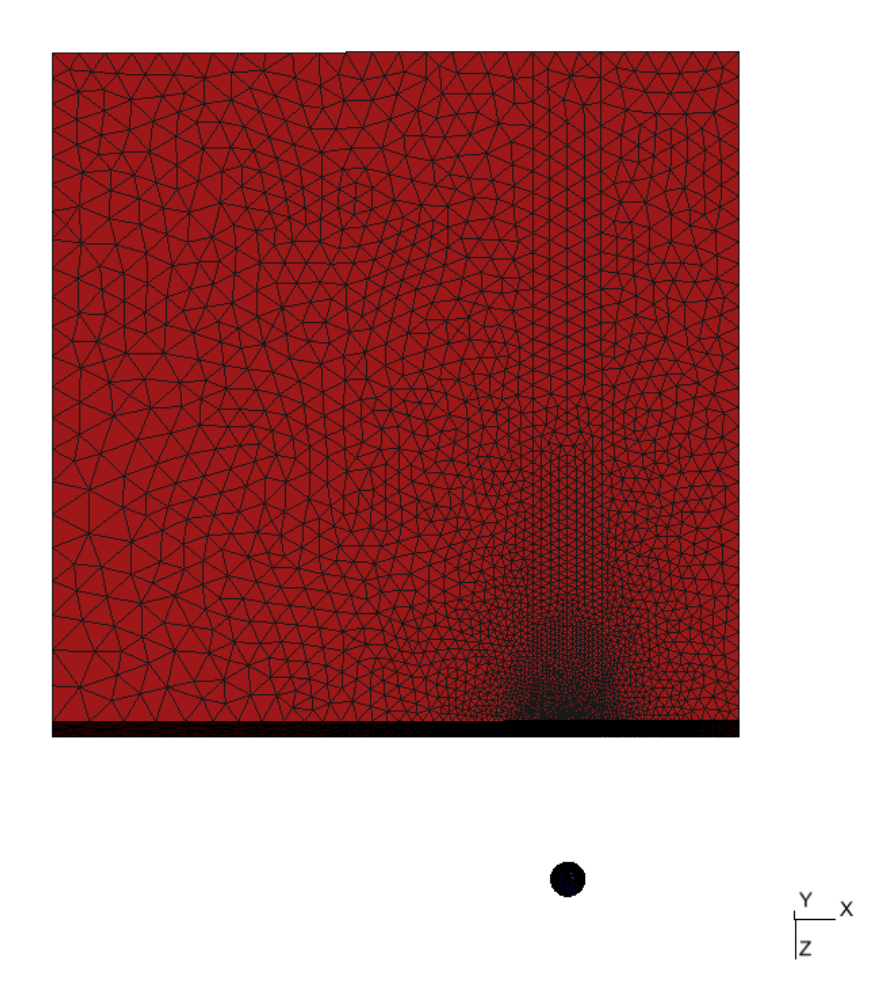
\includegraphics[height=3in]{L-20_W-25}
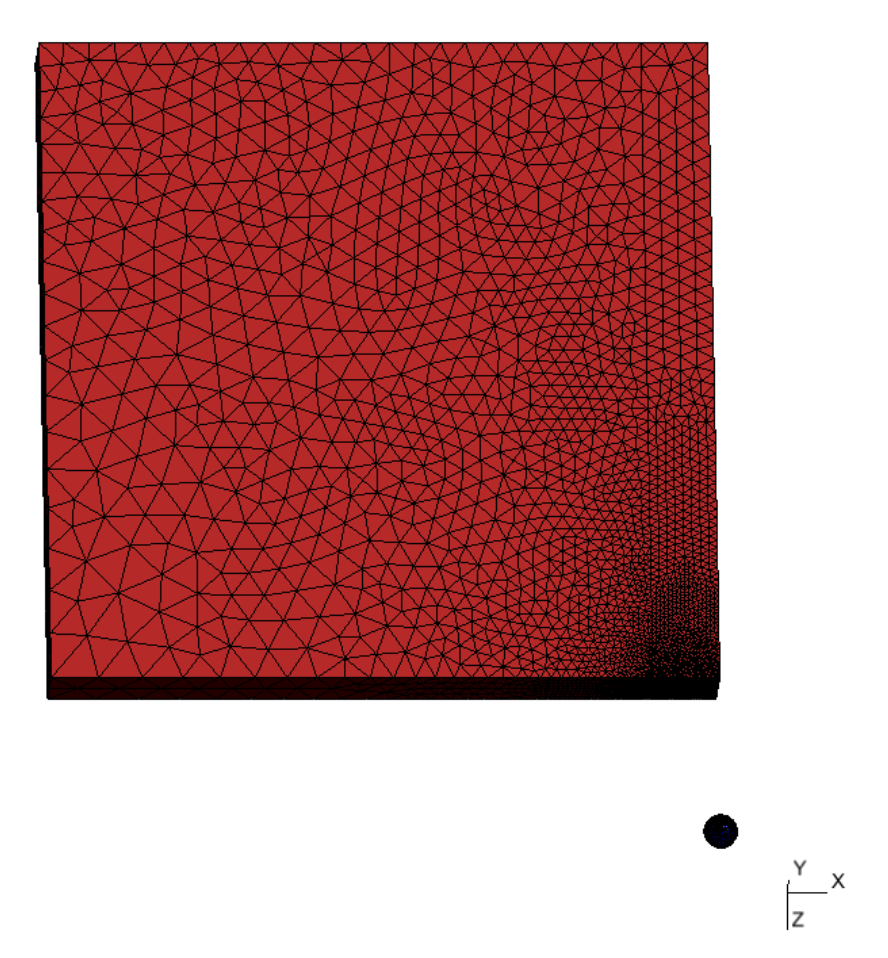
\includegraphics[height=3in]{L-20_W-50}
\caption{Geometry of cantilever and bead, representing the full x-y shape of the cantilever and extended to ~100 plasma wavelengths in depth. Here we show the bead 20 microns from the cantilever in the z direction, offset in the x direction by 25 and 50 microns. The radial meshing pattern has been made to follow to preserve convergence properties of the simulation/maximize accuracy nearest the sphere.}\label{fig:geoLat}
\end{figure}

\pagebreak
I created a geometry of a slab and sphere, both gridded finest nearest to each other with gridding decreasing on far surfaces. The sphere had gridding with a length scale twice as large on the back than the front, while the plane consisted of a uniformly gridded square nearest the sphere, and gridding decreasing as a function of distance from the square. I allowed the width, depth, and relative gridding on the far side of the cantilever to vary in order to test geometric convergence properties. Prediction as a function of plane width can be seen in figures \ref{fig:aspect} and \ref{fig:aspectFinite}, and we see that we need to simulate the full plane width (aspect ratio of 10) to get an accurate prediction; we cannot truncate this dimension. Prediction as a function of plane depth and rear gridding can be seen in figures \ref{fig:depth} and \ref{fig:depthCorr}, showing we need to simulate at least out to 100 microns in depth but can grid coarsely.

Based on these considerations, the final geometry I chose is a slab 100 microns by 100 microns by 10 microns in height as shown in figure \ref{fig:geoLarge}. For predictions as a function of displacement along the cantilever, I created a version which moves the finely gridded section laterally with the sphere, as shown in figure \ref{fig:geoLat}. In addition, the best gridding was a mesh length scale of 0.3 near the center. The numerical calculations for finite and infinite conductivities as well as 0 and finite temperature can be seen in figure \ref{fig:estimate}, compared to the analytic solutions from the previous section. In addition the simulations for lateral displacement along the cantilever can be seen in figures \ref{fig:lat}, \ref{fig:latdrop}, \ref{fig:latdropZoom}. These figures show a relatively constant force until the edge of the cantilever, where there's a rapid drop-off in force.

\begin{figure}[h]
\centering
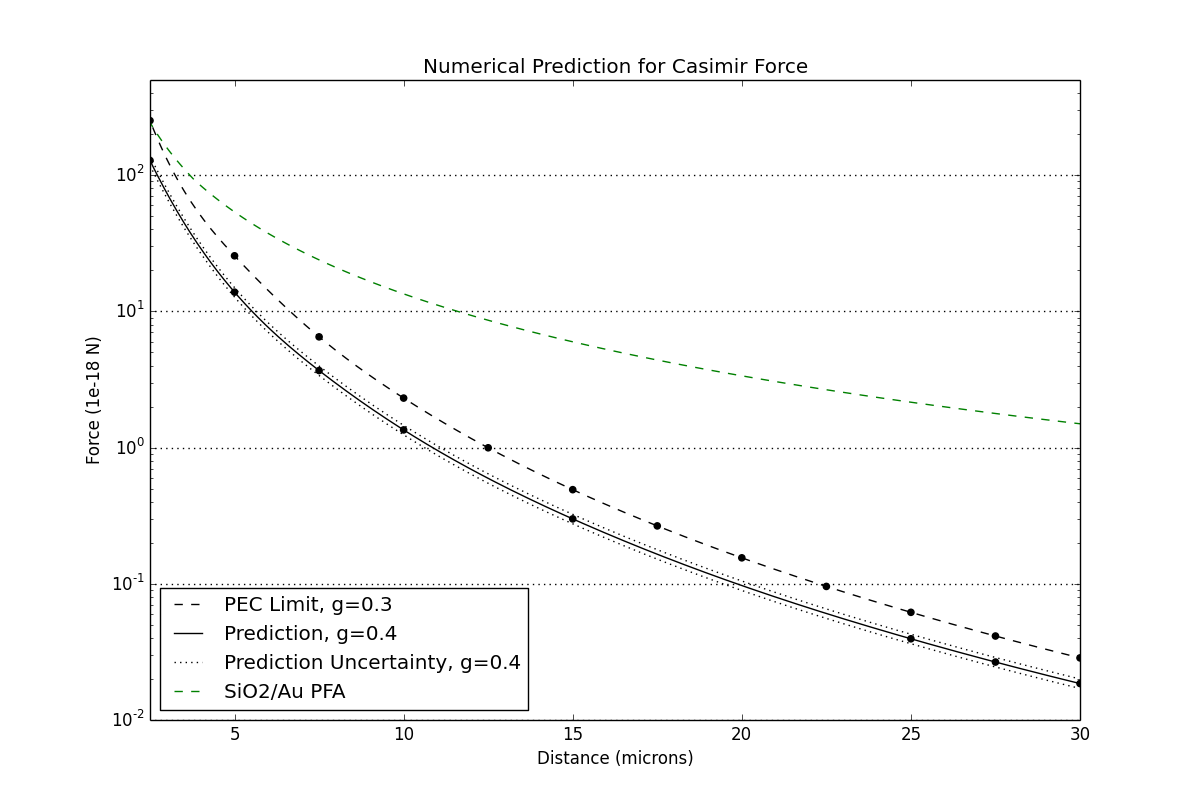
\includegraphics[width=7in]{prediction}
\caption{Best prediction for Casimir force at 300K with finite conductivity correction.}\label{fig:prediction}
\end{figure}

\begin{table}[h]
\centering
\begin{tabular}{c | c || c | c}
D ($\mu$m) & F (aN) &D ($\mu$m) & F (aN) \\
\hline
   3 & 7.37e+01 &  16 & 2.34e-01 \\
   4 & 2.90e+01 & 17 & 1.85e-01 \\
   5 & 1.38e+01 &  18 & 1.47e-01 \\
   6 & 7.61e+00 &  19 & 1.19e-01 \\
   7 & 4.61e+00 & 20 & 9.71e-02 \\
   8 & 2.96e+00 &  21 & 7.99e-02 \\
   9 & 1.97e+00 &  22 & 6.63e-02 \\
  10 & 1.35e+00 &  23 & 5.54e-02 \\
  11 & 9.53e-01 & 24 & 4.66e-02 \\
  12 & 6.92e-01 &  25 & 3.95e-02 \\
  13 & 5.14e-01 &  26 & 3.36e-02 \\
  14 & 3.89e-01 & 27 & 2.87e-02 \\
  15 & 3.00e-01 & 28 & 2.47e-02 \\
   & & 29 & 2.13e-02 \\
   \hline
\end{tabular}
\caption{Force as function of distance, silica bead and gold cantilever, in microns and attonewtons respectively. This points interpolated between slightly sparser points (5,10,15,20,25,30 are exact calculations) and have relative uncertainty on the 10\% level to high confidence.}\label{tab:pred}
\end{table}

The predictions for the force from our true geometry for the bead positioned at the center of the cantilever as a function of face-to-face separation are shown in figure \ref{fig:prediction} and tabulated in table \ref{tab:pred}. The numerical predictions show good agreement with the analytic solutions, and there is an extra geometric correction due to non-infinite plane (see figure \ref{fig:geomCorr}) which make the numerical predictions smaller than the analytic calculations. Given the uncertainty in the conductivity model and the untested nature of these methods, at worst this is an order of magnitude estimate and at best carries an uncertainty around 10\%.

\clearpage
\appendix
\section{Additional Figures}

\begin{figure}[h]
\centering
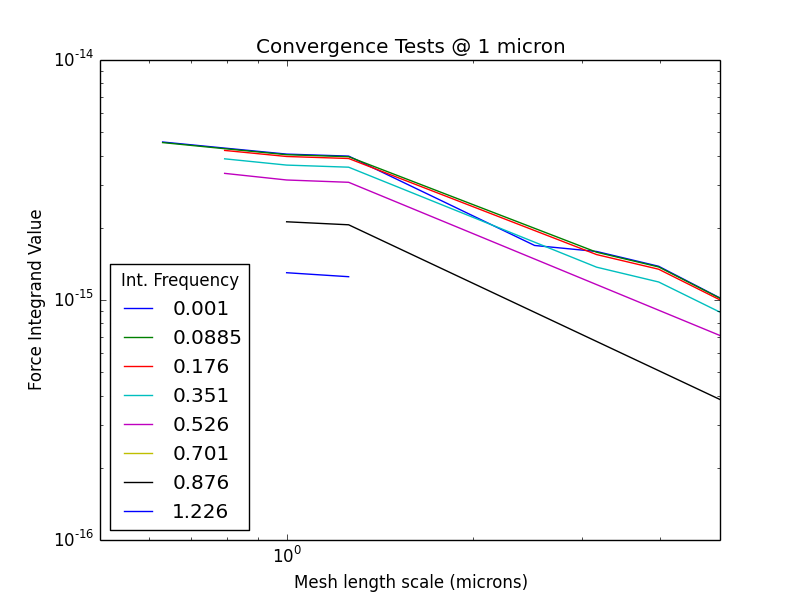
\includegraphics[width=5.5in]{convergence}
\caption{Earlier Casimir force estimates based on different geometries.}\label{fig:conv1}
\end{figure}

\begin{figure}[h]
\centering
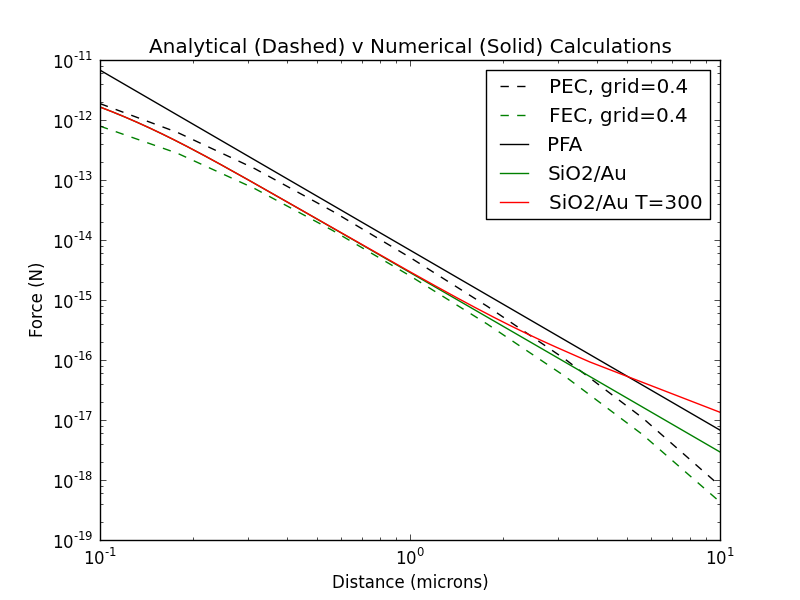
\includegraphics[width=7in]{analytic_v_numerical}
\caption{Earlier Casimir force estimates based on different geometries.}\label{fig:earlyEstimate}
\end{figure}

\begin{figure}[h]
\centering
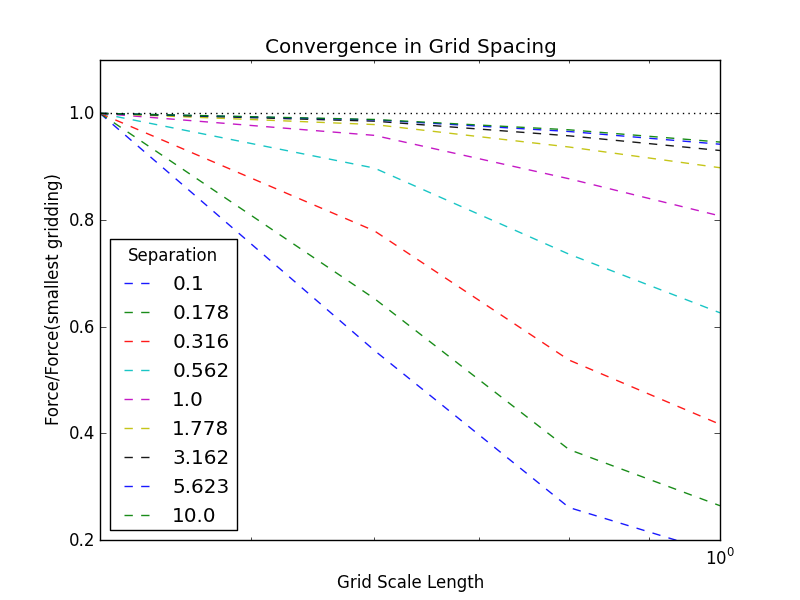
\includegraphics[width=5.5in]{pfa_convergence}
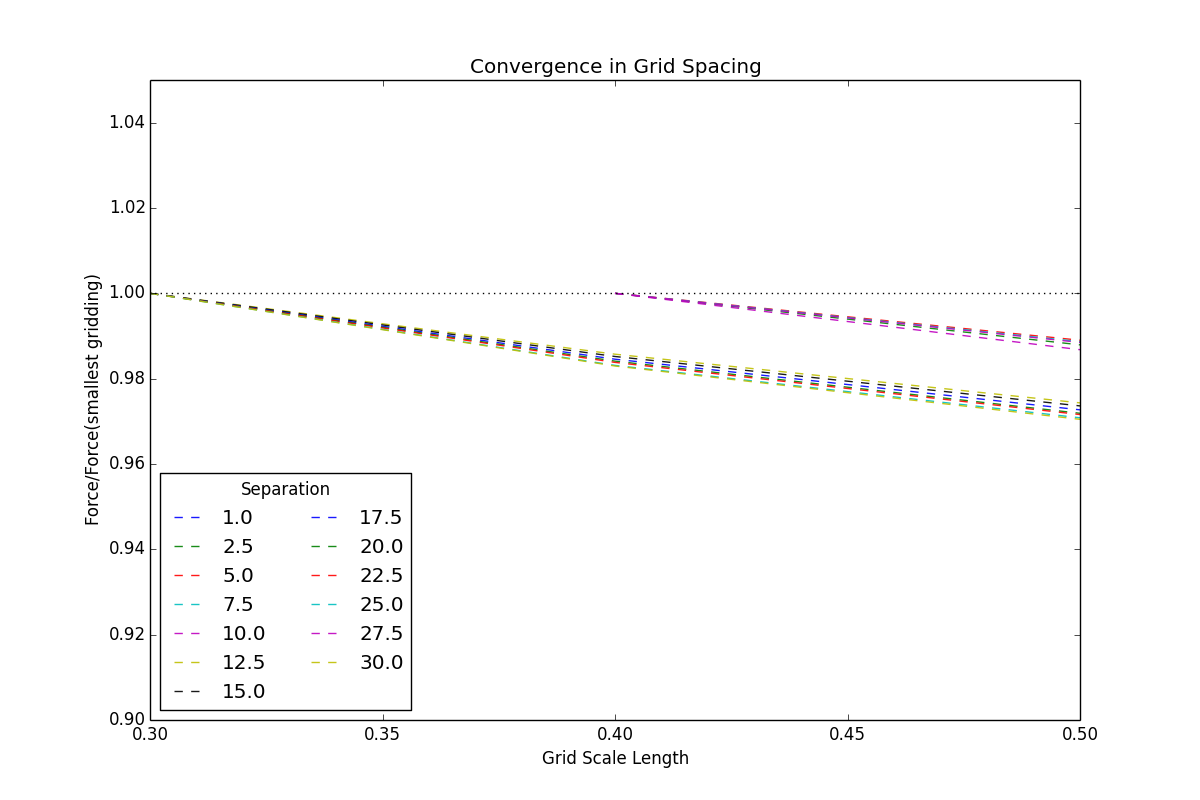
\includegraphics[width=5.5in]{pfa_convergence_zoom_best}
\caption{Convergence of numerical calculations as a function of separation and grid length scale for the small geometry (above) and full geometry (below).}\label{fig:conv2}
\end{figure}

\begin{figure}[h]
\centering
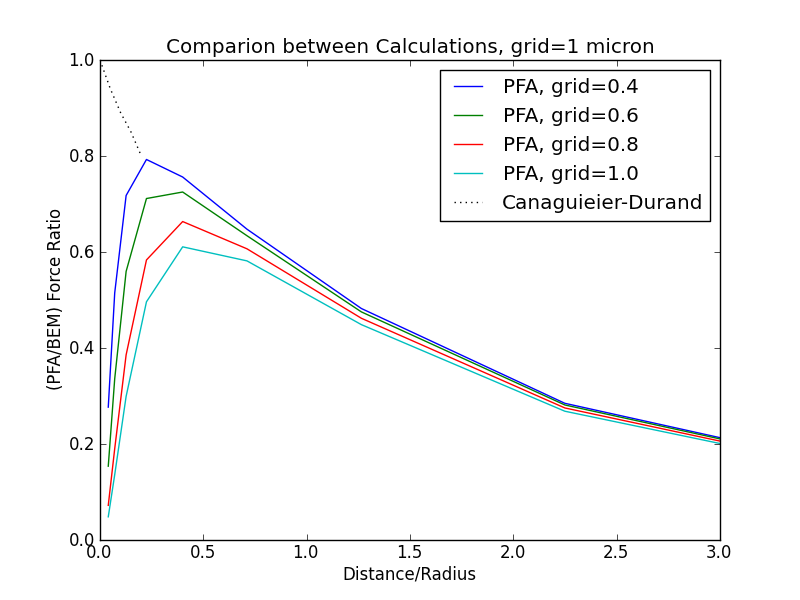
\includegraphics[width=7in]{pfa_v_pec}
\caption{PFA compared to numerical calculations.}\label{fig:geometric}
\end{figure}

\begin{figure}[h]
\centering
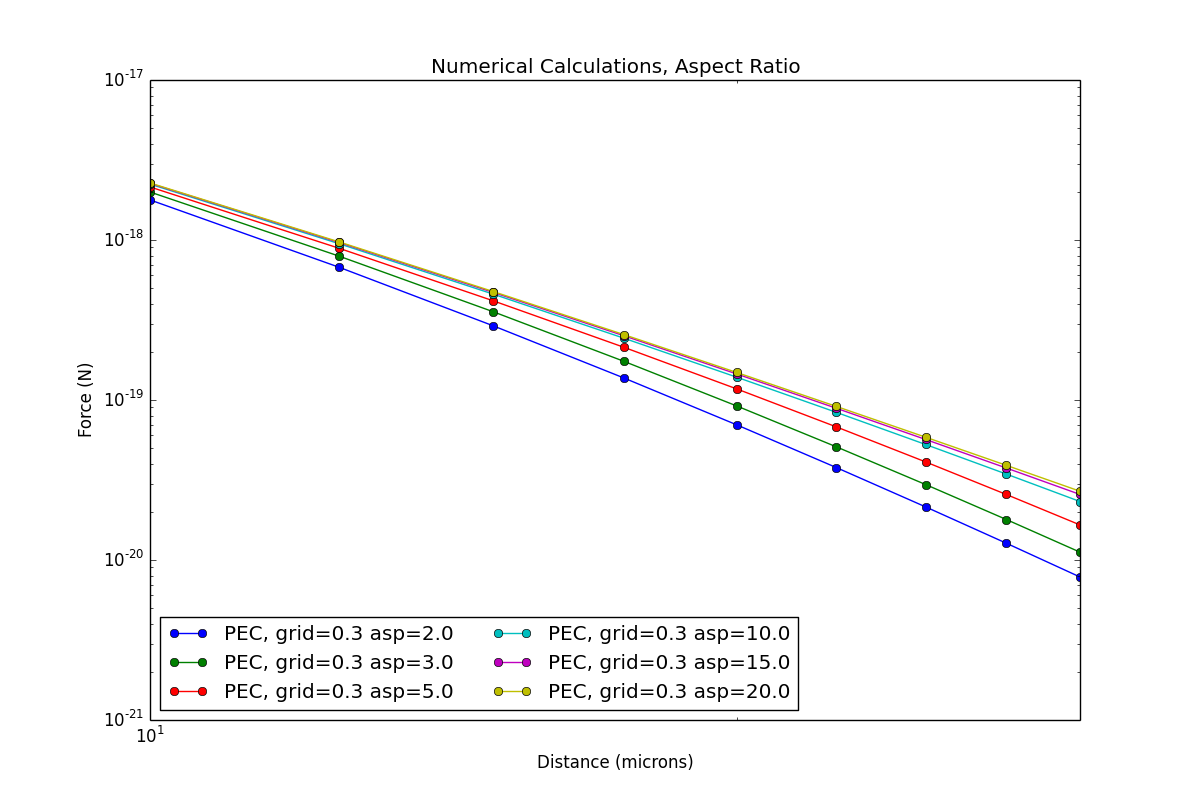
\includegraphics[width=5in]{force_v_aspect}
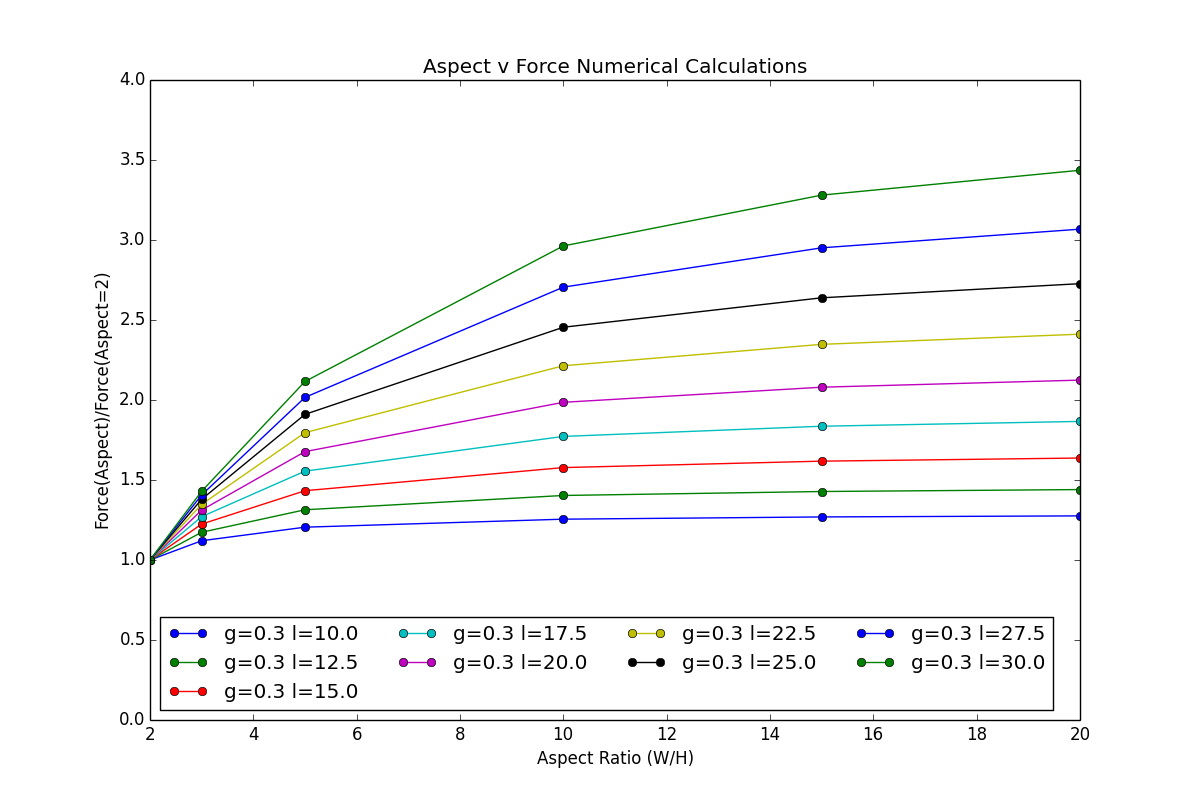
\includegraphics[width=5in]{aspect_correction}
\caption{Width (in terms of aspect ratio) versus distance from the cantilever for infinite conductivity and T=300K, showing increased variation of value from that at aspect ratio of 2 as separation increases (which makes sense geomertically). The cantilever we utilize corresponds to an aspect ratio of 10.}\label{fig:aspect}
\end{figure}

\begin{figure}[h]
\centering
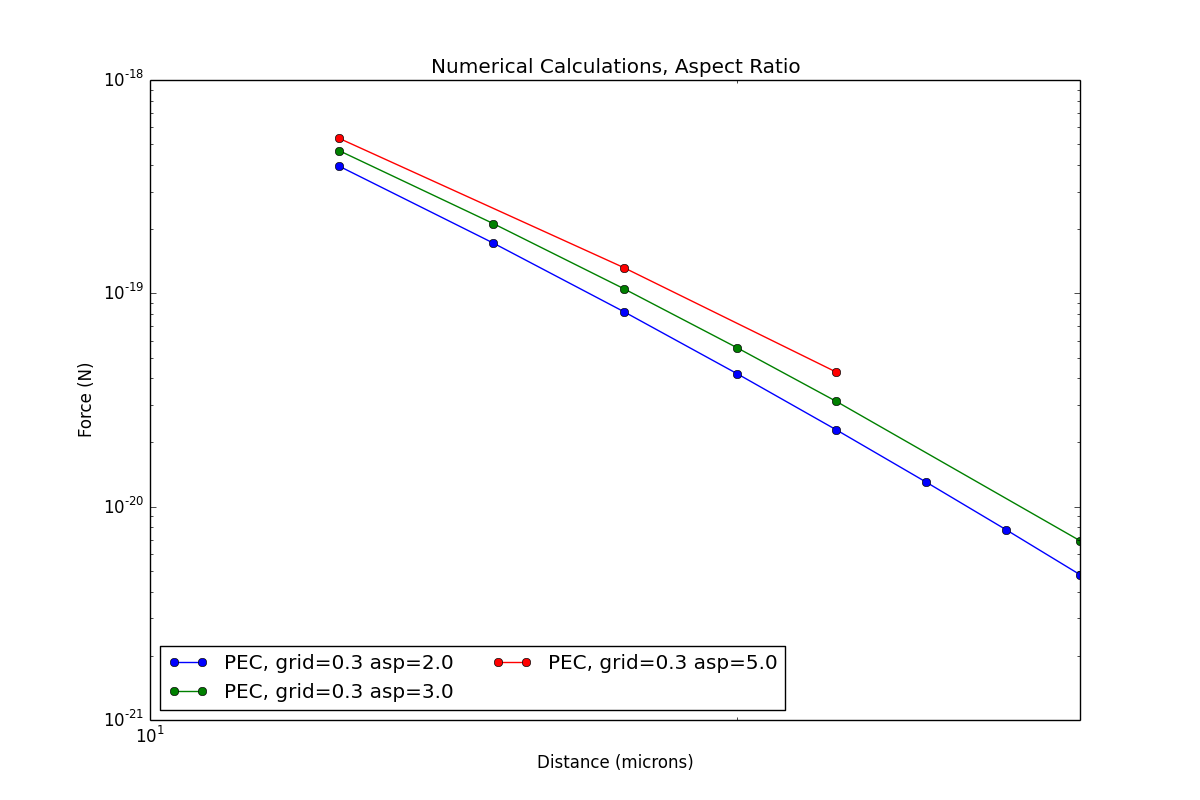
\includegraphics[width=5in]{force_v_aspect_finite}
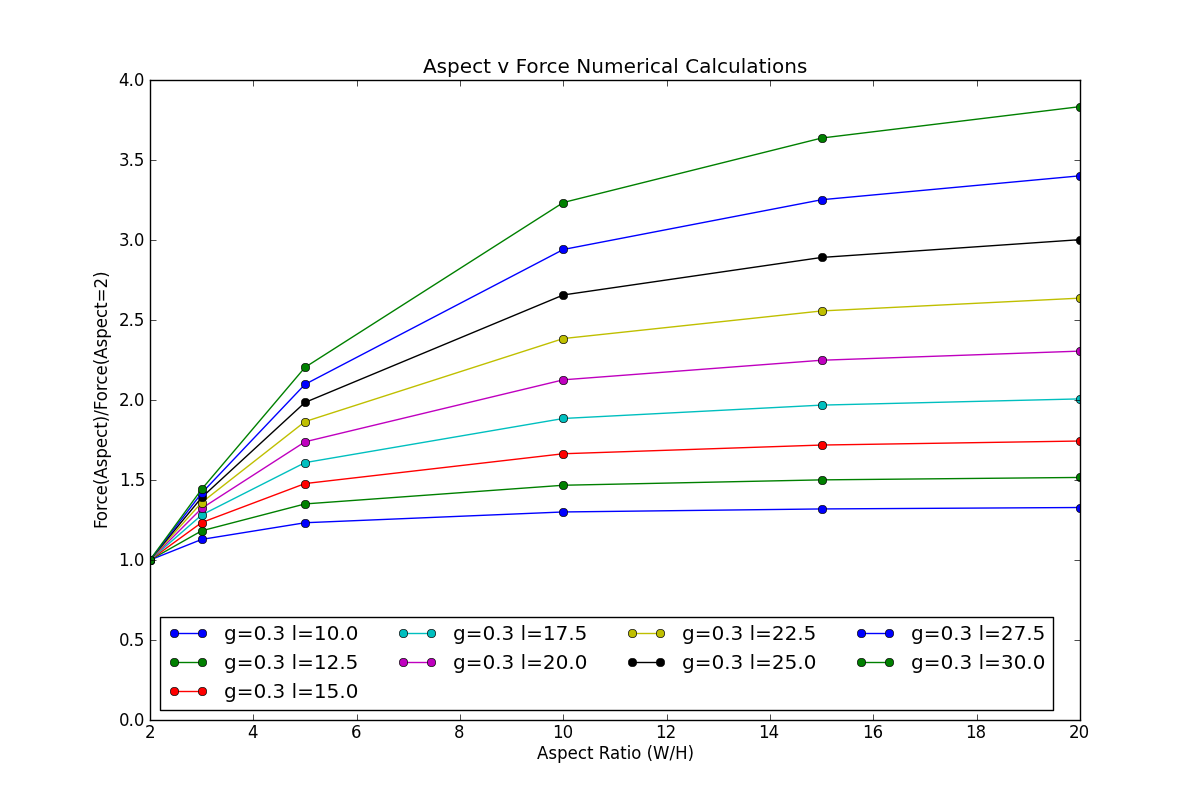
\includegraphics[width=5in]{aspect_correction_finite}
\caption{Width (in terms of aspect ratio) versus distance from the cantilever for finite conductivity and T=300K, showing increased variation of value from that at aspect ratio of 2 as separation increases (which makes sense geomertically). The cantilever we utilize corresponds to an aspect ratio of 10.}\label{fig:aspectFinite}
\end{figure}

\begin{figure}[h]
\centering
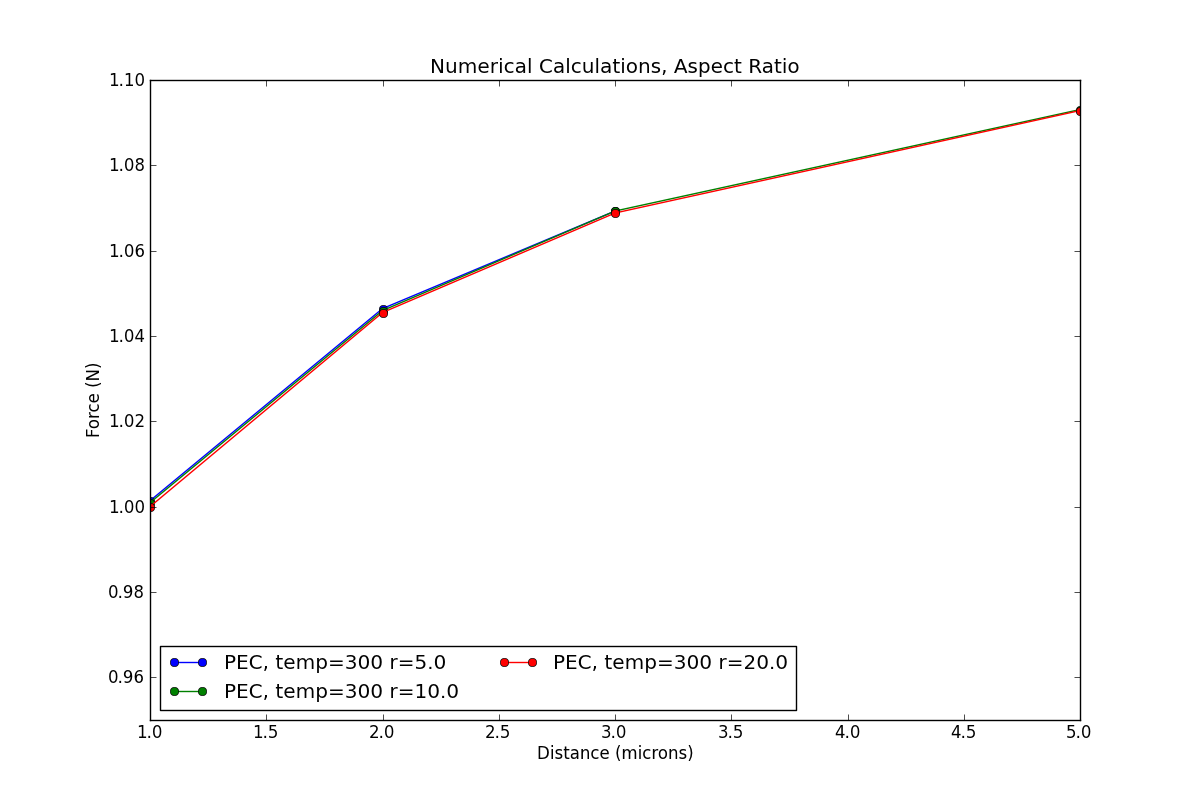
\includegraphics[width=5.5in]{depth_v_gridding}
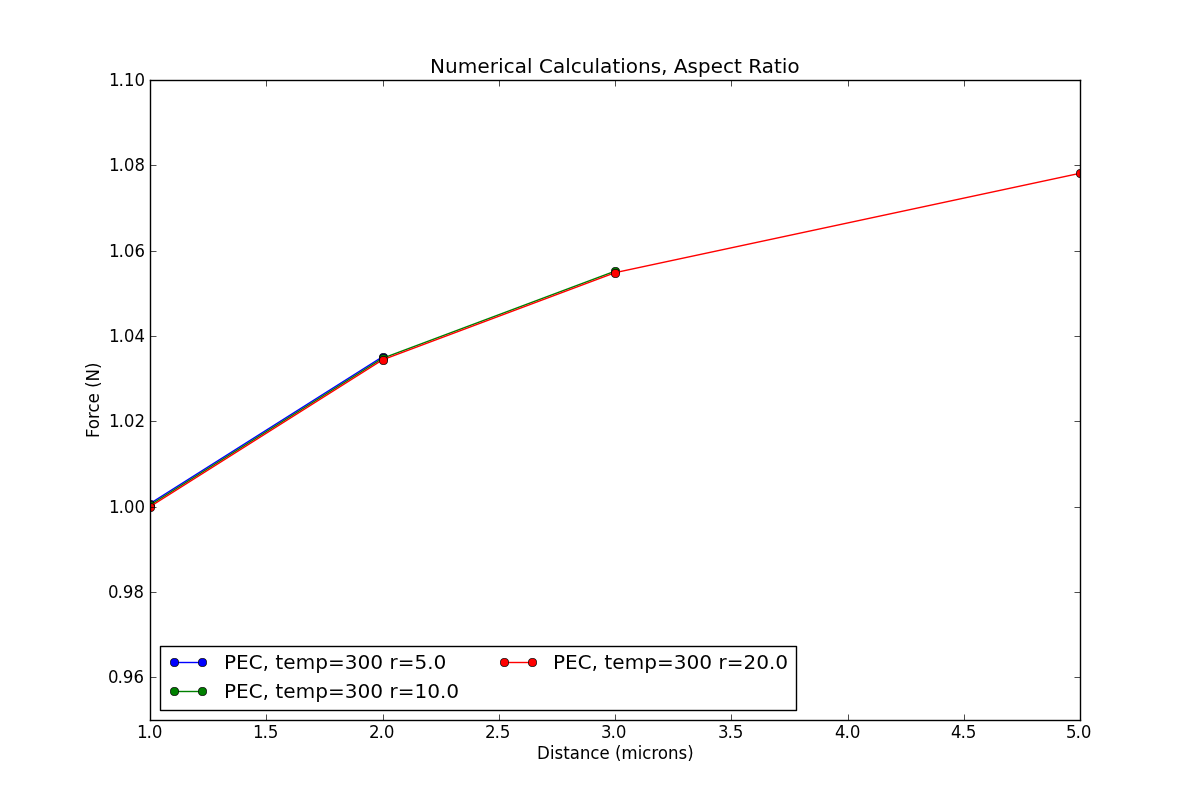
\includegraphics[width=5.5in]{depth_v_gridding_finite}
\caption{Depth versus relative grid size on the rear of the cantilever, showing relatively little dependence on relative grid size but large dependence on overall depth (fine gridding not as important as there being cells).}\label{fig:depth}
\end{figure}

\begin{figure}[h]
\centering
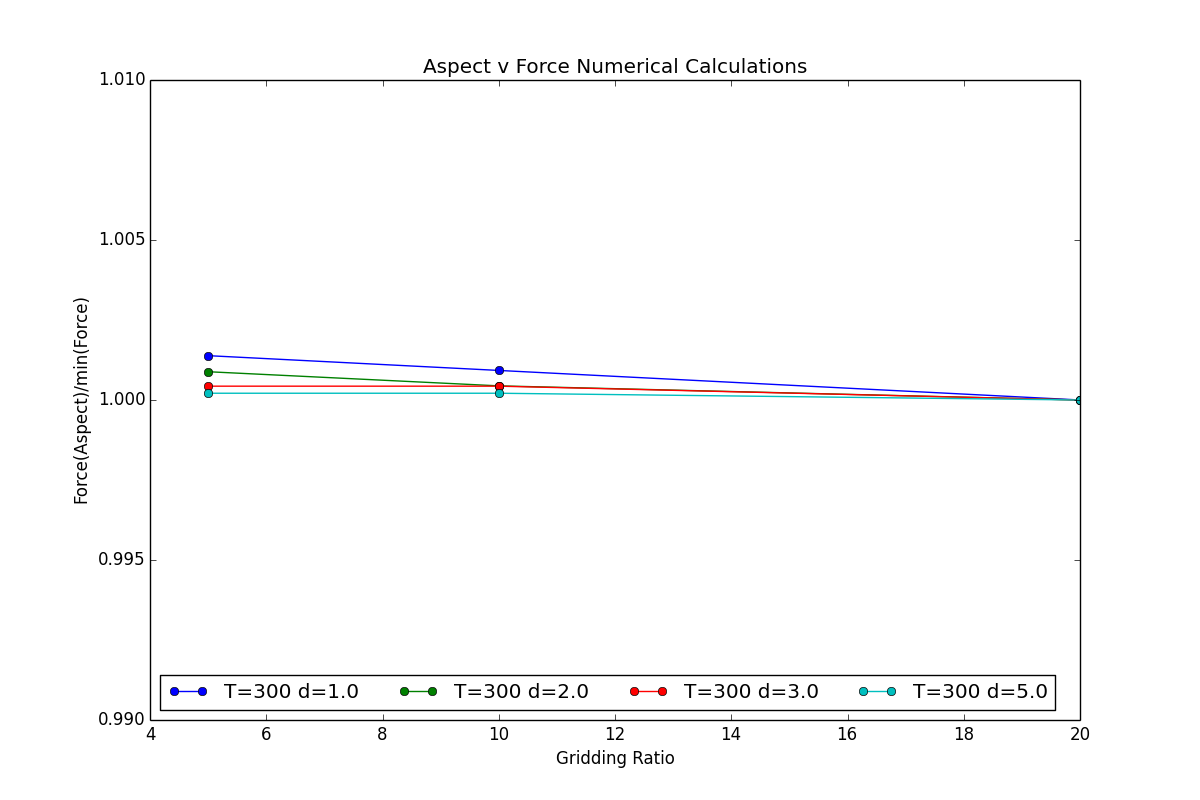
\includegraphics[width=5.5in]{depth_correction}
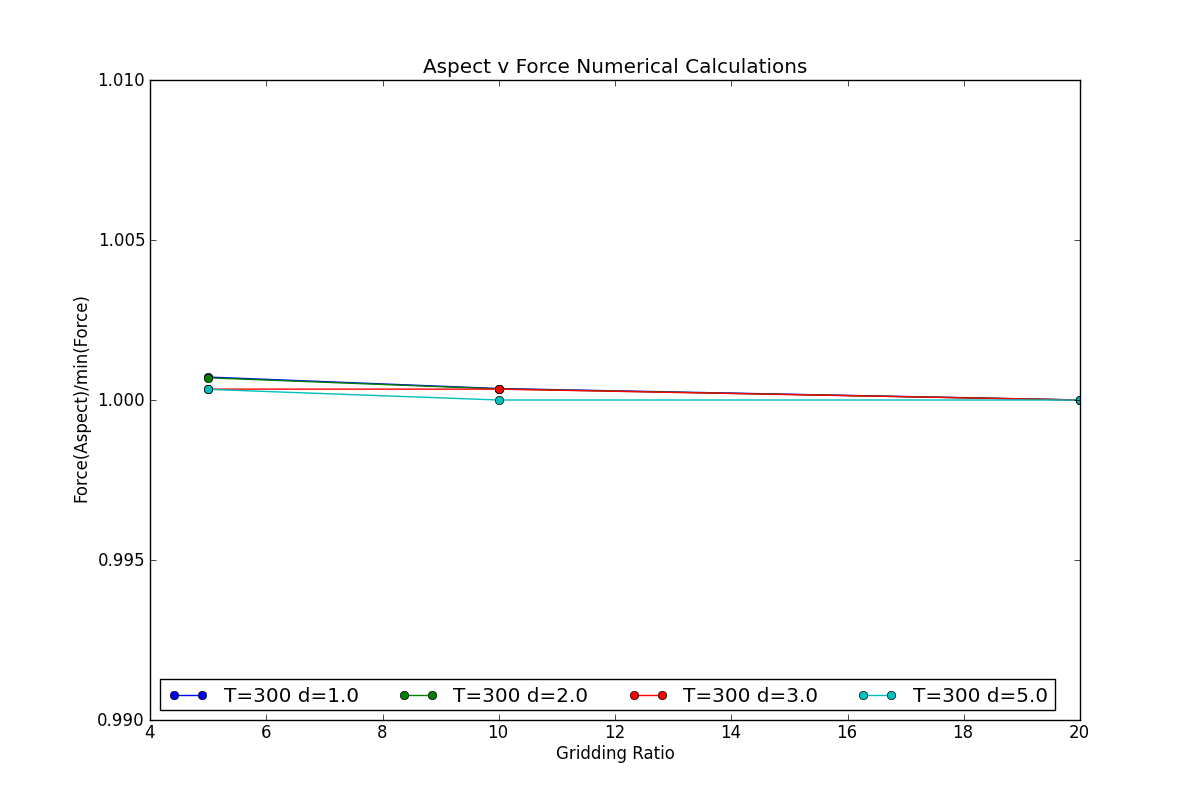
\includegraphics[width=5.5in]{depth_correction_finite}
\caption{Relative grid size on the rear of the cantilever versus force correction, showing relatively little dependence on relative grid size.}\label{fig:depthCorr}
\end{figure}

\begin{figure}[h]
\centering
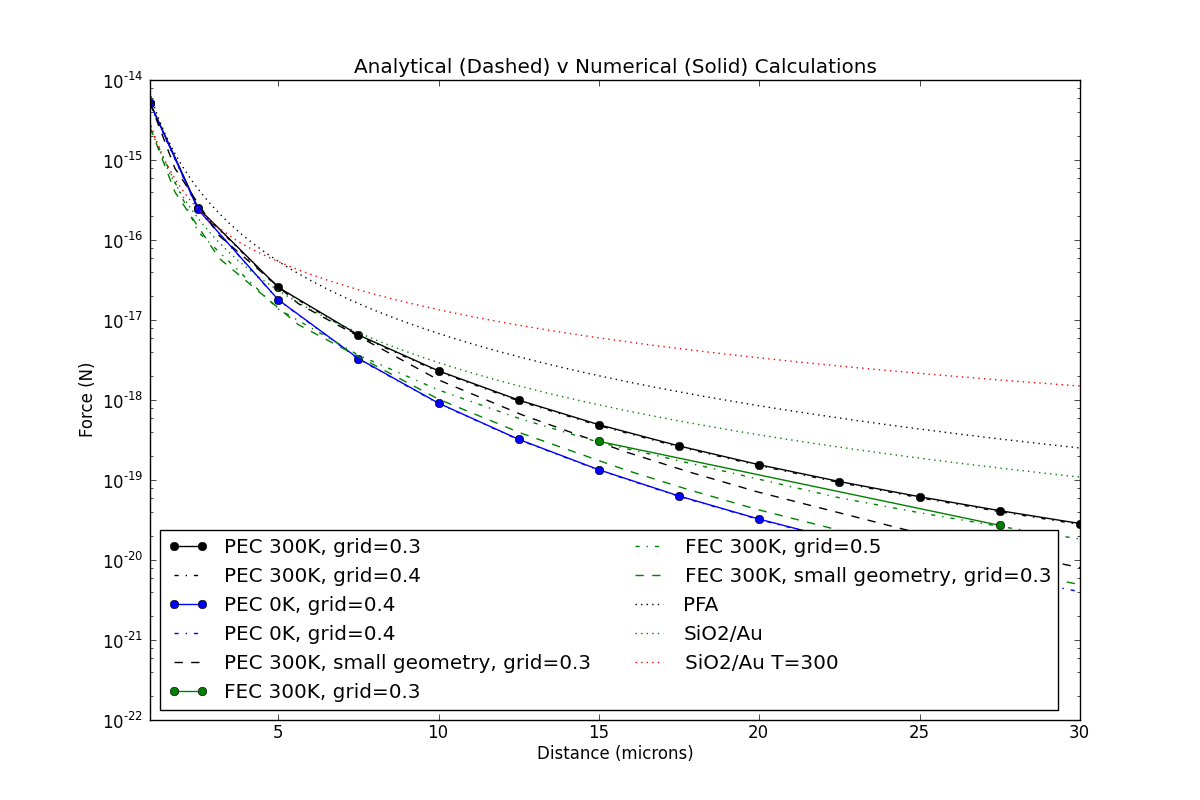
\includegraphics[width=7in]{analytic_v_numerical_best}
\caption{Casimir force estimate based on extended geometry.}\label{fig:estimate}
\end{figure}

\begin{figure}[h]
\centering
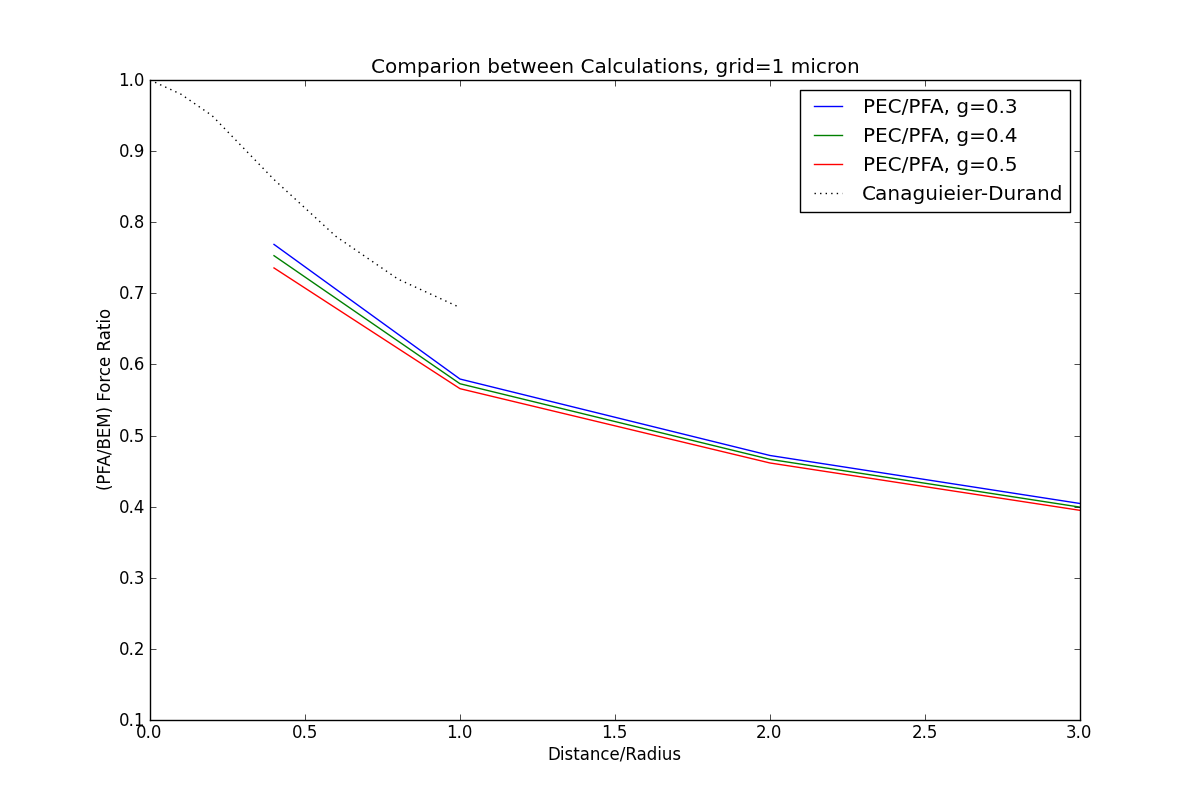
\includegraphics[width=5in]{pfa_v_pec_best}
\caption{Casimir force estimates compared to PFA, based on large geometry. Compared to correction for infinite plane.}\label{fig:geometricbest}
\end{figure}

\begin{figure}[!h]
\centering
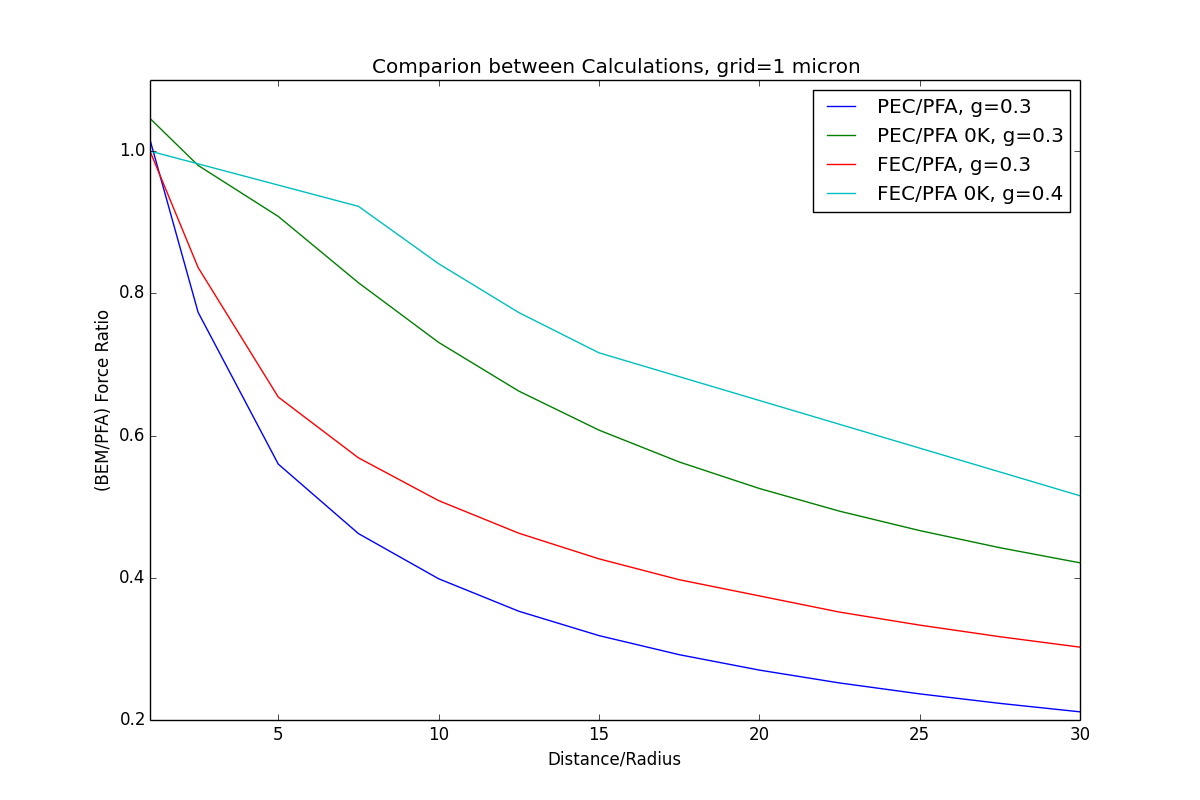
\includegraphics[width=5in]{geometry_corrections}
\caption{Full PFA expansion compared to numerical calculations.}\label{fig:geomCorr}
\end{figure}

\begin{figure}[h]
\centering
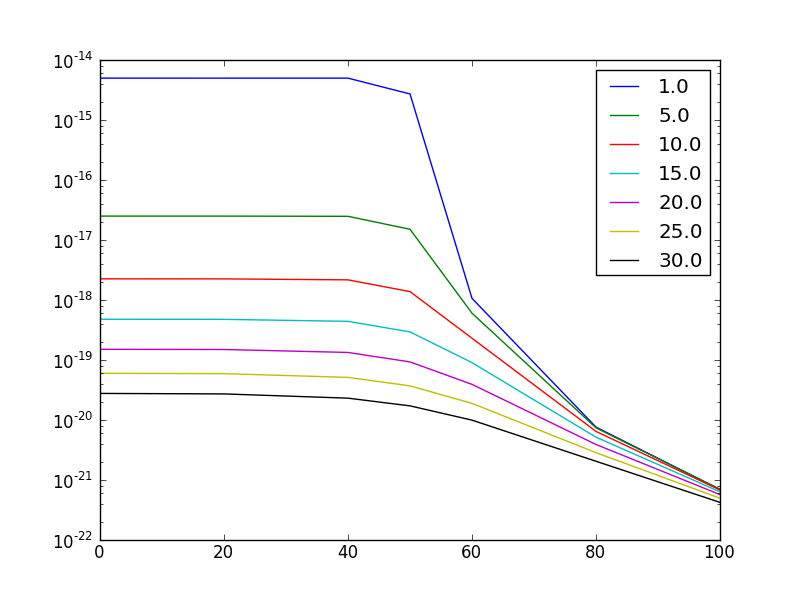
\includegraphics[width=5in]{lateral_force}
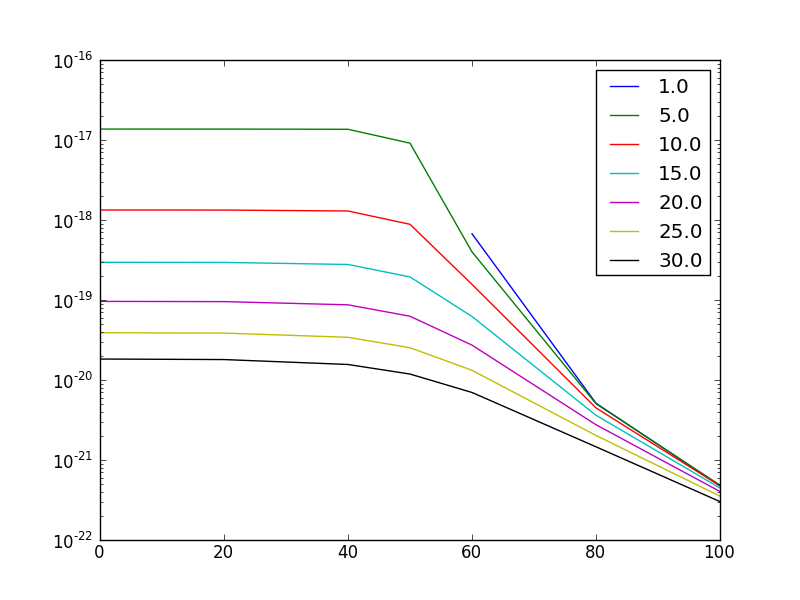
\includegraphics[width=5in]{lateral_force_finite}
\caption{Force as a function of lateral displacement along the cantilever for infinite (above) and finite (below) conductivity.}\label{fig:lat}
\end{figure}

\begin{figure}[h]
\centering
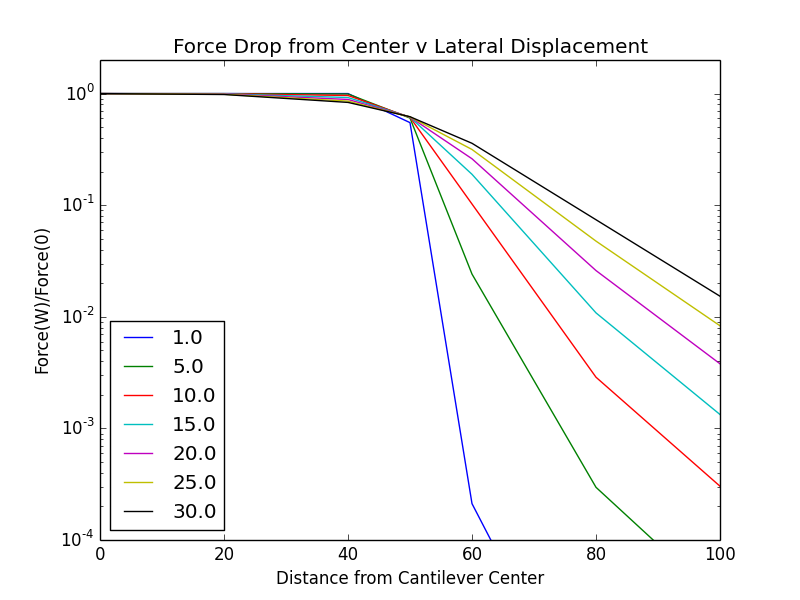
\includegraphics[width=5in]{lateral_force_drop}
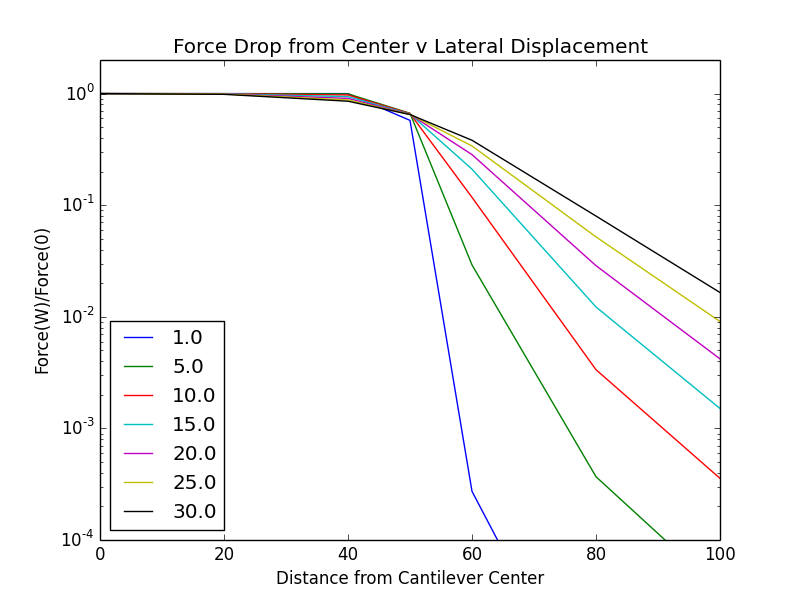
\includegraphics[width=5in]{lateral_force_drop_finite}
\caption{Force ratio as a function of lateral displacement along the cantilever for infinite (above) and finite (below) conductivity, as a fraction of the force near the center of the cantilever.}\label{fig:latdrop}
\end{figure}

\begin{figure}[h]
\centering
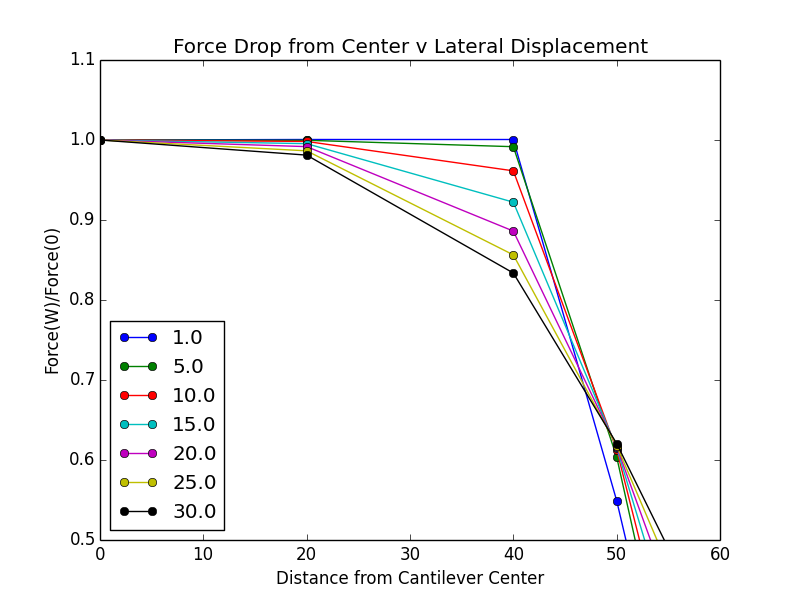
\includegraphics[width=5in]{lateral_force_drop_zoom}
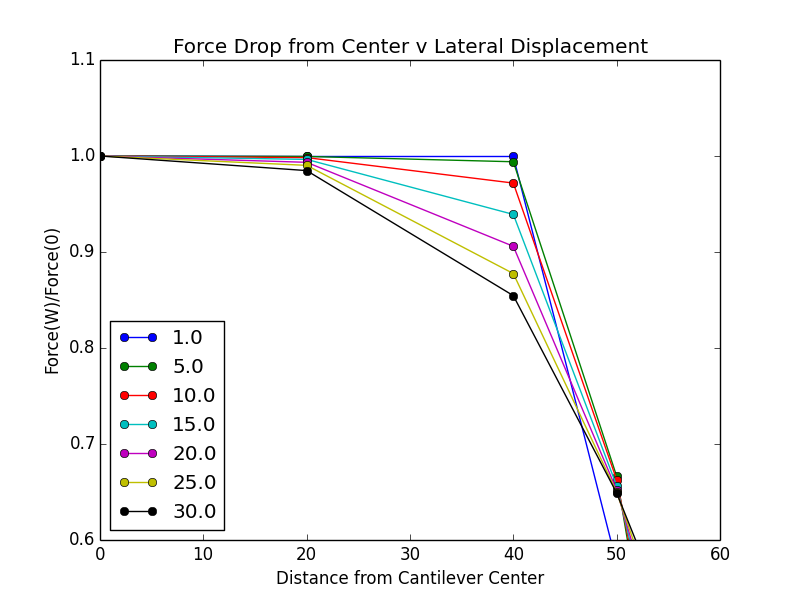
\includegraphics[width=5in]{lateral_force_drop_finite_zoom}
\caption{Force ratio as a function of lateral displacement along the cantilever for infinite (above) and finite (below) conductivity, as a fraction of the force near the center of the cantilever. Here we zoom in to capture the behavior near the cantilever edge}\label{fig:latdropZoom}
\end{figure}

\clearpage
\bibliographystyle{plainnat}
\bibliography{Casimir}
\thanks{here}

\end{document}  